\documentclass[12pt, oneside]{article}

\usepackage[letterpaper, scale=0.89, centering]{geometry}
\usepackage{fancyhdr}
\setlength{\parindent}{0em}
\setlength{\parskip}{1em}

\usepackage{tikz}
\usetikzlibrary{automata,positioning,arrows}

\pagestyle{fancy}
\fancyhf{}
\renewcommand{\headrulewidth}{0pt}
\rfoot{\href{https://creativecommons.org/licenses/by-nc-sa/2.0/}{CC BY-NC-SA 2.0} Version \today~(\thepage)}

\usepackage{amssymb,amsmath,pifont,amsfonts,comment,enumerate,enumitem}
\usepackage{currfile,xstring,hyperref,tabularx,graphicx,wasysym}
\usepackage[labelformat=empty]{caption}
\usepackage{xcolor}
\usepackage{multicol,multirow,array,listings,tabularx,lastpage,textcomp,booktabs}

\lstnewenvironment{algorithm}[1][] {   
    \lstset{ mathescape=true,
        frame=tB,
        numbers=left, 
        numberstyle=\tiny,
        basicstyle=\rmfamily\scriptsize, 
        keywordstyle=\color{black}\bfseries,
        keywords={,procedure, div, for, to, input, output, return, datatype, function, in, if, else, foreach, while, begin, end, }
        numbers=left,
        xleftmargin=.04\textwidth,
        #1
    }
}
{}

\newcommand\abs[1]{\lvert~#1~\rvert}
\newcommand{\st}{\mid}

\newcommand{\cmark}{\ding{51}}
\newcommand{\xmark}{\ding{55}}
 
\begin{document}
\begin{flushright}
    \StrBefore{\currfilename}{.}
\end{flushright} \section*{Week5 wednesday}


Warmup:   Design a CFG to generate the  language $\{a^i b^j \mid j \geq i  \geq 0\}$
  
\vfill
{\it Sample derivation:} 

\vspace{100pt}



Design a PDA to recognize the  language $\{a^i b^j \mid j \geq i  \geq 0\}$
  
\vspace{100pt}


\vfill
\newpage

{\bf Theorem  2.20}: A language is  generated by some context-free  grammar
if  and only if it is recognized by some push-down automaton.

Definition: a language is called {\bf context-free} if it is the language generated by a context-free grammar.
The class of all context-free language over a given alphabet $\Sigma$ is called {\bf CFL}.

Consequences:
\begin{itemize}
    \item Quick proof that every regular language is context free 
    \item To prove closure of the class of context-free languages under a given operation, we can choose 
    either of two modes 
    of proof (via CFGs or PDAs) depending on which is easier
    \item To fully specify a PDA we could give its $6$-tuple formal definition or we could give its input 
alphabet, stack alphabet, and state diagram.
An informal description of a PDA is a step-by-step description of how its computations 
would process input strings; the reader should be able to reconstruct the state diagram or formal 
definition precisely from such a descripton. The informal description of a PDA can refer to some 
common modules or subroutines that are computable by PDAs:
\begin{itemize}
  \item PDAs can ``test for emptiness of stack'' without providing details. 
  {\it How?} We can always push a special end-of-stack symbol, $\$$, at the start, before processing
  any input, and then use this symbol as a flag.
  \item PDAs can ``test for end of input'' without providing details.
  {\it How?} We can transform a PDA to one where accepting states are only those reachable 
  when there are no more input symbols.
\end{itemize}

\end{itemize}




\vfill

\newpage
Suppose $L_1$ and $L_2$ are context-free languages over $\Sigma$.  {\bf Goal}:  $L_1 \cup L_2$  is  also context-free.

{\it Approach 1: with  PDAs}

Let $M_1 = ( Q_1, \Sigma, \Gamma_1, \delta_1, q_1, F_1)$ and
$M_2 = ( Q_2, \Sigma, \Gamma_2, \delta_2, q_2, F_2)$ be PDAs with 
$L(M_1) =  L_1$  and  $L(M_2) = L_2$.

Define $M = $

\vfill

{\it Approach  2: with CFGs}

Let $G_1 = (V_1, \Sigma, R_1, S_1)$  and   $G_2 = (V_2, \Sigma, R_2, S_2)$  be CFGs  with
$L(G_1) =  L_1$  and  $L(G_2) = L_2$.

Define $G = $

\vfill

\newpage
Suppose $L_1$ and $L_2$ are context-free languages over $\Sigma$.  {\bf Goal}:  $L_1 \circ L_2$  is  also context-free.


{\it Approach 1: with  PDAs}

Let $M_1 = ( Q_1, \Sigma, \Gamma_1, \delta_1, q_1, F_1)$ and
$M_2 = ( Q_2, \Sigma, \Gamma_2, \delta_2, q_2, F_2)$ be PDAs with 
$L(M_1) =  L_1$  and  $L(M_2) = L_2$.

Define $M = $

\vfill

{\it Approach  2: with CFGs}

Let $G_1 = (V_1, \Sigma, R_1, S_1)$  and   $G_2 = (V_2, \Sigma, R_2, S_2)$  be CFGs  with
$L(G_1) =  L_1$  and  $L(G_2) = L_2$.

Define $G = $

\vfill
\newpage
{\it Summary}

Over a fixed alphabet $\Sigma$, a language $L$ is {\bf regular}

\vspace{-20pt}
\begin{center}
    iff it is described by some regular expression \\
    iff it is recognized by some DFA\\
    iff it is recognized by some NFA
\end{center}

Over a fixed alphabet $\Sigma$, a language $L$ is {\bf context-free}

\vspace{-20pt}
\begin{center}
    iff it is generated by some CFG\\
    iff it is recognized by some PDA
\end{center}

{\bf Fact}: Every regular language is a context-free language.

{\bf Fact}: There are context-free languages that are not nonregular.

{\bf Fact}: There are countably many regular languages.

{\bf Fact}: There are countably inifnitely many context-free languages.

{\it Consequence}: Most languages are {\bf not} context-free!

{\bf Examples  of non-context-free languages}

\begin{align*}
    &\{ a^n b^n c^n \mid 0 \leq n , n \in \mathbb{Z}\}\\
    &\{ a^i b^j c^k \mid 0 \leq i \leq j \leq k , i \in \mathbb{Z}, j \in \mathbb{Z}, k \in \mathbb{Z}\}\\
    &\{ ww \mid w \in \{0,1\}^* \}
\end{align*}
(Sipser Ex 2.36, Ex 2.37, 2.38)

There is a Pumping Lemma for CFL that can be used to prove a specific language is non-context-free: 
If $A$ is a context-free language, there there
is a number $p$ where, if $s$ is any string in $A$ of length at least $p$, then $s$ may be divided 
into five pieces $s = uvxyz$ where (1) for each $i \geq 0$, $uv^ixy^iz \in A$, (2) $|uv|>0$, (3) $|vxy| \leq p$.
{\it We will not go into the details of the proof or application of Pumping Lemma for CFLs this quarter.}

\begin{comment}
##Moved to review quiz
A set $X$ is said to be {\bf closed} under an operation $OP$ if, for any elements in $X$, applying 
$OP$ to them gives an element in $X$.  


\begin{center}
\begin{tabular}{|c|l|}
\hline
True/False & Closure claim \\
\hline
True &  The set of integers is closed under multiplication. \\
& $\forall x \forall y \left( ~(x \in \mathbb{Z} \wedge y \in \mathbb{Z})\to xy \in \mathbb{Z}~\right)$ \\
\hline
True & For each set $A$, the power set of $A$ is closed under intersection. \\
& $\forall A_1 \forall A_2 \left( ~(A_1 \in \mathcal{P}(A) \wedge A_2 \in \mathcal{P}(A) \in \mathbb{Z}) \to A_1 \cap A_2 \in \mathcal{P}(A)~\right)$ \\
\hline
  & The class of regular languages over $\Sigma$ is closed under complementation. \\
  & \\
 \hline
  & The class of regular languages over $\Sigma$ is closed under union. \\
  & \\
 \hline
  & The class of regular languages over $\Sigma$ is closed under intersection. \\
  & \\
  \hline
  & The class of regular languages over $\Sigma$ is closed under concatenation. \\
  & \\
 \hline
  & The class of regular languages over $\Sigma$ is closed under Kleene star. \\
  & \\
\hline
    & The class of context-free languages over $\Sigma$ is closed under complementation. \\
  & \\
\hline
    & The class of context-free languages over $\Sigma$ is closed under union. \\
  & \\
\hline
    & The class of context-free languages over $\Sigma$ is closed under intersection. \\
  & \\
\hline
    & The class of context-free languages over $\Sigma$ is closed under concatenation. \\
  & \\
\hline
    & The class of context-free languages over $\Sigma$ is closed under Kleene star. \\
  & \\
\hline
\end{tabular}
\end{center}
\end{comment}

 \vfill
\section*{Week5 friday}


 \vfill
\section*{Week4 wednesday}


Regular sets are not the end of the story
\begin{itemize}
    \item Many nice / simple / important sets are not regular
    \item Limitation of the finite-state automaton model: Can't ``count", Can only remember finitely far into the past,
    Can't backtrack, Must make decisions in ``real-time"
    \item We know actual computers are more powerful than this model...
\end{itemize}

The {\bf next} model of computation. Idea: allow some memory of unbounded size. How? 
\begin{itemize}
    \item To generalize regular expressions: {\bf context-free grammars}\\
    \item To generalize NFA: {\bf Pushdown automata}, which is like an NFA with access to a stack: 
    Number of states is fixed, number of entries in stack is unbounded. At each step
    (1) Transition to new state based on current state, letter read, and top letter of stack, then
    (2) (Possibly) push or pop a letter to (or from) top of stack. Accept a string iff
    there is some sequence of states and some sequence of stack contents 
    which helps the PDA processes the entire input string and ends in an accepting state.
\end{itemize}

\vfill

\vfill

Is there a PDA that recognizes the nonregular language $\{0^n1^n \mid n \geq 0 \}$?

\vfill

\newpage


\includegraphics[width=4in]{Lect9PDA.png}

The PDA with state diagram above can be informally described as:
\begin{quote}
    Read symbols from the input. As each 0 is read, push it onto the stack. 
    As soon as 1s are seen, pop a 0 off the stack for each 1 read. 
    If the stack becomes empty and we are at the end of the input string, accept the input. 
    If the stack becomes empty and there are 1s left to read, 
    or if 1s are finished while the stack still contains 0s, or if any 0s
    appear in the string following 1s, 
    reject the input.
\end{quote}
    

Trace the computation of this PDA on the input string $01$.

\vfill
    
Trace the computation of this PDA on the input string $011$.

\vfill

\newpage
A PDA recognizing the set $\{ \hspace{1.5 in} \}$ can be informally described as:
\begin{quote}
    Read symbols from the input. As each 0 is read, push it onto the stack. 
    As soon as 1s are seen, pop a 0 off the stack for each 1 read. 
    If the stack becomes empty and there is exactly one 1 left to read, read that 1 and accept the input. 
    If the stack becomes empty and there are either zero or more than one 1s left to read, 
    or if the 1s are finished while the stack still contains 0s, or if any 0s appear in the input following 1s, 
    reject the input.
\end{quote}
Modify the state diagram below to get a PDA that implements this description:

\includegraphics[width=4in]{Lect9PDA.png}


\vfill
{\bf Definition} A {\bf pushdown automaton} (PDA) is  specified by a  $6$-tuple $(Q, \Sigma, \Gamma, \delta, q_0, F)$
where $Q$ is the finite set of states, $\Sigma$ is the input alphabet,  $\Gamma$ is the stack alphabet,
\[
    \delta: Q \times \Sigma_\varepsilon  \times  \Gamma_\varepsilon \to \mathcal{P}( Q \times \Gamma_\varepsilon)
\]
is the transition function,  $q_0 \in Q$ is the start state, $F \subseteq  Q$ is the set of accept states.
    
 \vfill
\section*{Week4 friday}




Draw the state diagram and give the formal definition of a PDA with $\Sigma = \Gamma$.

\vfill

Draw the state diagram and give the formal definition of a PDA with $\Sigma \cap \Gamma = \emptyset$.
    
\vfill

\newpage
For the PDA state diagrams below, $\Sigma = \{0,1\}$.


\begin{center}
\begin{tabular}{c c}
Mathematical description of language & State diagram of PDA recognizing language\\
\hline
& $\Gamma = \{ \$, \#\}$ \hspace{2.3in} \\
& \\
& \includegraphics[width=3.5in]{Lect10PDA1.png}\\
& \\
& \\
\hline
& $\Gamma = \{ {@}, 1\}$ \hspace{2.3in} \\
& \\
& \includegraphics[width=3.5in]{Lect10PDA2.png}\\
& \\
& \\
\hline
& \\
& \\
& \\
$\{ 0^i 1^j 0^k \mid i,j,k \geq 0 \}$ & \\
& \\
& \\
\end{tabular}
\end{center}

 \vfill
 {\it Note: alternate notation is to replace $;$ with $\to$}

\begin{comment}
{\it Extra practice}: Consider the state diagram of a PDA with input alphabet 
$\Sigma$ and stack alphabet $\Gamma$.

\begin{center}
\begin{tabular}{|c|c|}
\hline
Label & means \\
\hline
$a, b ; c$ when $a \in \Sigma$, $b\in \Gamma$, $c \in \Gamma$ 
& \hspace{3in} \\
& \\
& \\
& \\
& \\
&\\
\hline
$a, \varepsilon ; c$ when $a \in \Sigma$, $c \in \Gamma$ 
& \hspace{3in} \\
& \\
& \\
& \\
& \\
&\\
\hline
$a, b ; \varepsilon$ when $a \in \Sigma$, $b\in \Gamma$
& \hspace{3in} \\
& \\
& \\
& \\
& \\
&\\
\hline
$a, \varepsilon ; \varepsilon$ when $a \in \Sigma$
& \hspace{3in} \\
& \\
& \\
& \\
& \\
&\\
\hline
\end{tabular}
\end{center}


How does the meaning change if $a$ is replaced by $\varepsilon$?
\end{comment}


{\it Big picture}: PDAs were motivated by wanting to add some memory of unbounded size to NFA. How 
do we accomplish a similar enhancement of regular expressions to get a syntactic model that is 
more expressive?

DFA, NFA, PDA: Machines process one input string at a time; the computation of a machine on its input string 
reads the input from left to right.

Regular expressions: Syntactic descriptions of all strings that match a particular pattern; the language 
described by a regular expression is built up recursively according to the expression's syntax

{\bf Context-free grammars}: Rules to produce one string at a time, adding characters from the middle, beginning, 
or end of the final string as the derivation proceeds.

 \vfill
\section*{Week6 monday}


For Turing machine $M= (Q, \Sigma, \Gamma, \delta, q_0, q_{accept}, q_{reject})$ 
where $\delta$ is the {\bf transition function} 
\[
  \delta: Q\times \Gamma \to Q \times \Gamma \times \{L, R\}
\]
the {\bf computation} of $M$ on a string $w$ over $\Sigma$  is:

\begin{itemize}
\setlength{\itemsep}{0pt}
\item Read/write head starts at leftmost position on tape. 
\item Input string is written on $|w|$-many leftmost cells of tape, 
rest of  the tape cells have  the blank symbol. {\bf Tape alphabet} 
is $\Gamma$ with $\textvisiblespace\in \Gamma$ and $\Sigma \subseteq \Gamma$.
The blank symbol $\textvisiblespace \notin \Sigma$.
\item Given current state of machine and current symbol being read at the tape head, 
the machine transitions to next state, writes a symbol to the current position  of the 
tape  head (overwriting existing symbol), and moves the tape head L or R (if possible). 
\item Computation ends {\bf if and when} machine enters either the accept or the reject state.
This is called {\bf halting}.
Note: $q_{accept} \neq q_{reject}$.
\end{itemize}

The {\bf language recognized by the  Turing machine} $M$,  is  $L(M) = \{ w \in \Sigma^* \mid w \textrm{ is accepted by } M\}$,
which is defined as
\[
  \{ w \in \Sigma^* \mid \textrm{computation of $M$ on $w$ halts after entering the accept state}\}
\]
  
\newpage
\begin{multicols}{2}
\includegraphics[width=2.5in]{Lect13TM1.png}

\columnbreak
Formal definition:

\vspace{10pt}

Sample computation: 

\begin{tabular}{|c|c|c|c|c|c|c|}
\hline
\multicolumn{1}{|c}{$q0\downarrow$} &  \multicolumn{6}{c|}{\phantom{A}}\\
\hline
$0$ & $0$  & $0$ & $\textvisiblespace $& $\textvisiblespace $& $\textvisiblespace $&  $\textvisiblespace $\\
\hline
\multicolumn{7}{|c|}{\phantom{A}}\\
\hline
\phantom{AA} & \phantom{AA}& \phantom{AA}& \phantom{AA}& \phantom{AA}& \phantom{AA}& \phantom{AA} \\
\hline
\multicolumn{7}{|c|}{\phantom{A}}\\
\hline
\phantom{AA} & \phantom{AA}& \phantom{AA}& \phantom{AA}& \phantom{AA}& \phantom{AA}& \phantom{AA} \\
\hline
\multicolumn{7}{|c|}{\phantom{A}}\\
\hline
\phantom{AA} & \phantom{AA}& \phantom{AA}& \phantom{AA}& \phantom{AA}& \phantom{AA}& \phantom{AA} \\
\hline
\multicolumn{7}{|c|}{\phantom{A}}\\
\hline
\phantom{AA} & \phantom{AA}& \phantom{AA}& \phantom{AA}& \phantom{AA}& \phantom{AA}& \phantom{AA} \\
\hline
\end{tabular}
\end{multicols}
\vfill

The language recognized by this machine is \ldots

\vfill


To define a Turing machine, we could give a 
\begin{itemize}
\item {\bf Formal definition}, namely the $7$-tuple of parameters including set of states, 
input alphabet, tape alphabet, transition function, start state, accept state, and reject state; or,
\item {\bf Implementation-level definition}: English prose that describes the Turing machine head 
movements relative to contents of tape, and conditions for accepting / rejecting based on those contents.
\end{itemize}

Conventions for drawing state diagrams of Turing machines: (1) omit the reject state from the diagram (unless 
it's the  start state), (2) any missing transitions in the state diagram have value $(q_{reject}, ~\textvisiblespace~ , R)$.
\newpage

{\it Sipser Figure  3.10}
\begin{multicols}{2}
\vspace{-20pt}
\begin{center}
\includegraphics[width=4in]{Lect13TM3.png}
\end{center}

Implementation level description of this machine:
\begin{quote}
Zig-zag across tape to corresponding positions on either side of $\#$ to check whether the 
characters in these positions agree. If they do not, or if there is no $\#$, reject. If they 
do, cross them off.

Once all symbols to the left of the $\#$ are crossed off, check for any un-crossed-off symbols 
to the right of $\#$; if there are any, reject; if there aren't, accept.
\end{quote}

\columnbreak

Computation on  input  string  $01\#01$

\begin{tabular}{|c|c|c|c|c|c|c|}
\hline
\multicolumn{1}{|c}{$q_1 \downarrow$} &  \multicolumn{6}{c|}{\phantom{A}}\\
\hline
$0$ & $1$  & $\#$  & $0$ & $1$ & $\textvisiblespace $& $\textvisiblespace $\\
\hline
  \multicolumn{7}{|c|}{\phantom{A}}\\
  \hline
  \phantom{AA} & \phantom{AA}& \phantom{AA}& \phantom{AA}& \phantom{AA}& \phantom{AA}& \phantom{AA} \\
  \hline
  \multicolumn{7}{|c|}{\phantom{A}}\\
  \hline
  \phantom{AA} & \phantom{AA}& \phantom{AA}& \phantom{AA}& \phantom{AA}& \phantom{AA}& \phantom{AA} \\
  \hline
  \multicolumn{7}{|c|}{\phantom{A}}\\
  \hline
  \phantom{AA} & \phantom{AA}& \phantom{AA}& \phantom{AA}& \phantom{AA}& \phantom{AA}& \phantom{AA} \\
  \hline
  \multicolumn{7}{|c|}{\phantom{A}}\\
  \hline
  \phantom{AA} & \phantom{AA}& \phantom{AA}& \phantom{AA}& \phantom{AA}& \phantom{AA}& \phantom{AA} \\
  \hline
  \multicolumn{7}{|c|}{\phantom{A}}\\
  \hline
  \phantom{AA} & \phantom{AA}& \phantom{AA}& \phantom{AA}& \phantom{AA}& \phantom{AA}& \phantom{AA} \\
  \hline
  \multicolumn{7}{|c|}{\phantom{A}}\\
  \hline
  \phantom{AA} & \phantom{AA}& \phantom{AA}& \phantom{AA}& \phantom{AA}& \phantom{AA}& \phantom{AA} \\
  \hline
  \multicolumn{7}{|c|}{\phantom{A}}\\
  \hline
  \phantom{AA} & \phantom{AA}& \phantom{AA}& \phantom{AA}& \phantom{AA}& \phantom{AA}& \phantom{AA} \\
  \hline
  \multicolumn{7}{|c|}{\phantom{A}}\\
  \hline
  \phantom{AA} & \phantom{AA}& \phantom{AA}& \phantom{AA}& \phantom{AA}& \phantom{AA}& \phantom{AA} \\
  \hline
  \multicolumn{7}{|c|}{\phantom{A}}\\
  \hline
  \phantom{AA} & \phantom{AA}& \phantom{AA}& \phantom{AA}& \phantom{AA}& \phantom{AA}& \phantom{AA} \\
  \hline
  \multicolumn{7}{|c|}{\phantom{A}}\\
  \hline
  \phantom{AA} & \phantom{AA}& \phantom{AA}& \phantom{AA}& \phantom{AA}& \phantom{AA}& \phantom{AA} \\
  \hline
  \multicolumn{7}{|c|}{\phantom{A}}\\
  \hline
  \phantom{AA} & \phantom{AA}& \phantom{AA}& \phantom{AA}& \phantom{AA}& \phantom{AA}& \phantom{AA} \\
  \hline
  \multicolumn{7}{|c|}{\phantom{A}}\\
  \hline
  \phantom{AA} & \phantom{AA}& \phantom{AA}& \phantom{AA}& \phantom{AA}& \phantom{AA}& \phantom{AA} \\
  \hline
  \multicolumn{7}{|c|}{\phantom{A}}\\
  \hline
  \phantom{AA} & \phantom{AA}& \phantom{AA}& \phantom{AA}& \phantom{AA}& \phantom{AA}& \phantom{AA} \\
  \hline
  \multicolumn{7}{|c|}{\phantom{A}}\\
  \hline
  \phantom{AA} & \phantom{AA}& \phantom{AA}& \phantom{AA}& \phantom{AA}& \phantom{AA}& \phantom{AA} \\
  \hline
  \multicolumn{7}{|c|}{\phantom{A}}\\
  \hline
  \phantom{AA} & \phantom{AA}& \phantom{AA}& \phantom{AA}& \phantom{AA}& \phantom{AA}& \phantom{AA} \\
  \hline
  \multicolumn{7}{|c|}{\phantom{A}}\\
  \hline
  \phantom{AA} & \phantom{AA}& \phantom{AA}& \phantom{AA}& \phantom{AA}& \phantom{AA}& \phantom{AA} \\
  \hline
  \multicolumn{7}{|c|}{\phantom{A}}\\
  \hline
  \phantom{AA} & \phantom{AA}& \phantom{AA}& \phantom{AA}& \phantom{AA}& \phantom{AA}& \phantom{AA} \\
  \hline
  \multicolumn{7}{|c|}{\phantom{A}}\\
  \hline
  \phantom{AA} & \phantom{AA}& \phantom{AA}& \phantom{AA}& \phantom{AA}& \phantom{AA}& \phantom{AA} \\
  \hline
  \end{tabular}
\end{multicols}


The language recognized by this machine is
\[
  \{ w \# w \mid w \in \{0,1\}^* \}
\]

\newpage
{\it Extra practice}

Computation on  input  string  $01\#1$

\begin{tabular}{|c|c|c|c|c|c|c|}
\hline
\multicolumn{1}{|c}{$q_1\downarrow$} &  \multicolumn{6}{c|}{\phantom{A}}\\
\hline
$0$ & $1$  & $\#$  & $1$ & $\textvisiblespace $& $\textvisiblespace $&  $\textvisiblespace $\\
\hline
\multicolumn{7}{|c|}{\phantom{A}}\\
\hline
\phantom{AA} & \phantom{AA}& \phantom{AA}& \phantom{AA}& \phantom{AA}& \phantom{AA}& \phantom{AA} \\
\hline
\multicolumn{7}{|c|}{\phantom{A}}\\
\hline
\phantom{AA} & \phantom{AA}& \phantom{AA}& \phantom{AA}& \phantom{AA}& \phantom{AA}& \phantom{AA} \\
\hline
\multicolumn{7}{|c|}{\phantom{A}}\\
\hline
\phantom{AA} & \phantom{AA}& \phantom{AA}& \phantom{AA}& \phantom{AA}& \phantom{AA}& \phantom{AA} \\
\hline
\multicolumn{7}{|c|}{\phantom{A}}\\
\hline
\phantom{AA} & \phantom{AA}& \phantom{AA}& \phantom{AA}& \phantom{AA}& \phantom{AA}& \phantom{AA} \\
\hline
\multicolumn{7}{|c|}{\phantom{A}}\\
\hline
\phantom{AA} & \phantom{AA}& \phantom{AA}& \phantom{AA}& \phantom{AA}& \phantom{AA}& \phantom{AA} \\
\hline
\multicolumn{7}{|c|}{\phantom{A}}\\
\hline
\phantom{AA} & \phantom{AA}& \phantom{AA}& \phantom{AA}& \phantom{AA}& \phantom{AA}& \phantom{AA} \\
\hline
\multicolumn{7}{|c|}{\phantom{A}}\\
\hline
\phantom{AA} & \phantom{AA}& \phantom{AA}& \phantom{AA}& \phantom{AA}& \phantom{AA}& \phantom{AA} \\
\hline
\multicolumn{7}{|c|}{\phantom{A}}\\
\hline
\phantom{AA} & \phantom{AA}& \phantom{AA}& \phantom{AA}& \phantom{AA}& \phantom{AA}& \phantom{AA} \\
\hline
\multicolumn{7}{|c|}{\phantom{A}}\\
\hline
\phantom{AA} & \phantom{AA}& \phantom{AA}& \phantom{AA}& \phantom{AA}& \phantom{AA}& \phantom{AA} \\
\hline
\multicolumn{7}{|c|}{\phantom{A}}\\
\hline
\phantom{AA} & \phantom{AA}& \phantom{AA}& \phantom{AA}& \phantom{AA}& \phantom{AA}& \phantom{AA} \\
\hline
\multicolumn{7}{|c|}{\phantom{A}}\\
\hline
\phantom{AA} & \phantom{AA}& \phantom{AA}& \phantom{AA}& \phantom{AA}& \phantom{AA}& \phantom{AA} \\
\hline
\multicolumn{7}{|c|}{\phantom{A}}\\
\hline
\phantom{AA} & \phantom{AA}& \phantom{AA}& \phantom{AA}& \phantom{AA}& \phantom{AA}& \phantom{AA} \\
\hline
\multicolumn{7}{|c|}{\phantom{A}}\\
\hline
\phantom{AA} & \phantom{AA}& \phantom{AA}& \phantom{AA}& \phantom{AA}& \phantom{AA}& \phantom{AA} \\
\hline
\multicolumn{7}{|c|}{\phantom{A}}\\
\hline
\phantom{AA} & \phantom{AA}& \phantom{AA}& \phantom{AA}& \phantom{AA}& \phantom{AA}& \phantom{AA} \\
\hline
\multicolumn{7}{|c|}{\phantom{A}}\\
\hline
\phantom{AA} & \phantom{AA}& \phantom{AA}& \phantom{AA}& \phantom{AA}& \phantom{AA}& \phantom{AA} \\
\hline
\multicolumn{7}{|c|}{\phantom{A}}\\
\hline
\phantom{AA} & \phantom{AA}& \phantom{AA}& \phantom{AA}& \phantom{AA}& \phantom{AA}& \phantom{AA} \\
\hline
\multicolumn{7}{|c|}{\phantom{A}}\\
\hline
\phantom{AA} & \phantom{AA}& \phantom{AA}& \phantom{AA}& \phantom{AA}& \phantom{AA}& \phantom{AA} \\
\hline
\multicolumn{7}{|c|}{\phantom{A}}\\
\hline
\phantom{AA} & \phantom{AA}& \phantom{AA}& \phantom{AA}& \phantom{AA}& \phantom{AA}& \phantom{AA} \\
\hline
\multicolumn{7}{|c|}{\phantom{A}}\\
\hline
\phantom{AA} & \phantom{AA}& \phantom{AA}& \phantom{AA}& \phantom{AA}& \phantom{AA}& \phantom{AA} \\
\hline
\multicolumn{7}{|c|}{\phantom{A}}\\
\hline
\phantom{AA} & \phantom{AA}& \phantom{AA}& \phantom{AA}& \phantom{AA}& \phantom{AA}& \phantom{AA} \\
\hline
\end{tabular}

 \vfill
\section*{Week6 wednesday}



  
  Fix $\Sigma = \{0,1\}$, $\Gamma = \{ 0, 1, \textvisiblespace\}$ for the Turing machines with  the following state diagrams:
  
  \begin{center}
  \begin{tabular}{|c|c|}
  \hline
  \hspace{0.8in}\includegraphics[width=2in]{Lect14TM1.png} \phantom{\hspace{0.8in}}&\hspace{0.8in} \includegraphics[width=2in]{Lect14TM2.png} \phantom{\hspace{0.8in}}\\
  Implementation  level description:  \phantom{\hspace{1in}} &Implementation  level description:  \phantom{\hspace{1in}} \\
  &\\
  &\\
  &\\
  Example of string accepted: \phantom{\hspace{1.5in}}& Example of string accepted: \phantom{\hspace{1.5in}}\\
  Example of string rejected: \phantom{\hspace{1.5in}}& Example of string  rejected: \phantom{\hspace{1.5in}}\\
  & \\
  \hline
  \includegraphics[width=2in]{Lect14TM3.png} & \includegraphics[width=2in]{Lect14TM4.png} \\
  Implementation  level description:  \phantom{\hspace{1in}} &Implementation  level description:  \phantom{\hspace{1in}} \\
  &\\
  &\\
  &\\
  Example of string accepted: \phantom{\hspace{1.5in}}& Example of string accepted: \phantom{\hspace{1.5in}}\\
  Example of string rejected: \phantom{\hspace{1.5in}}& Example of string  rejected: \phantom{\hspace{1.5in}}\\
  & \\
  
  \hline
  \end{tabular}
  \end{center}

Two models of computation are called {\bf equally expressive} when 
every language recognizable with the first model is recognizable with the second, and vice versa.

True / False: NFAs and PDAs are equally expressive.

True / False: Regular expressions and CFGs are equally expressive.


To say a language is {\bf Turing-recognizable} means that there is some Turing machine that recognizes it.

\begin{center}
{\large \it  Some examples of models that are {\bf equally expressive} with deterministic Turing machines: }
\end{center}

\newpage
\fbox{ {\bf May-stay}  machines }
The May-stay machine model is the same as the usual Turing machine model,  except that
on each transition, the tape head may move L, move R, or Stay. 

Formally: $(Q, \Sigma, \Gamma, \delta, q_0, q_{accept}, q_{reject})$ where 
\[
  \delta: Q \times \Gamma \to Q \times \Gamma \times \{L, R, S\}
\]

{\bf Claim}: Turing machines and May-stay machines are equally expressive. {\it To prove \ldots}

To translate a standard TM to a may-stay machine: 

\vspace{100pt}




To translate one  of the  may-stay machines to standard TM:
any time TM would Stay, move right  then  left.


Formally: suppose $M_S =  (Q, \Sigma, \Gamma, \delta, q_0, q_{acc}, q_{rej})$
has $\delta: Q \times \Gamma \to Q \times \Gamma \times \{L, R, S\}$. Define
the Turing-machine
\[
  M_{new} =  (\phantom{\hspace{2.5in}})
\]

\vfill


\phantom{$M_{new}$ construction here \vspace{400pt}}
\vfill

\newpage

\fbox{ {\bf Multitape Turing machine}} A multitape Turing macihne with $k$ tapes
can be formally representated as 
$(Q, \Sigma,  \Gamma, \delta, q_0, q_{acc}, q_{rej})$ 
where $Q$ is the finite set of  states,
$\Sigma$ is the  input alphabet with  $\textvisiblespace \notin \Sigma$,
$\Gamma$  is the  tape alphabet with $\Sigma \subsetneq \Gamma$ ,
$\delta: Q\times \Gamma^k\to Q \times \Gamma^k \times \{L,R\}^k$ 
(where $k$ is  the number of  states)


If $M$ is a standard  TM, it is a $1$-tape machine.


To translate a $k$-tape machine  to  a standard TM:
Use a  new symbol to separate the contents of each tape
and keep track of location of  head with  special version of each
tape symbol. {\tiny Sipser Theorem 3.13} 

\includegraphics[width=2.5in]{resources/images/Figure314.png}

\vfill

{\it Extra practice:} \fbox{ {\bf  Wikipedia Turing machine} }
Define a machine $(Q, \Gamma, b, \Sigma,  q_0, F, \delta)$
where $Q$ is the finite set  of  states
$\Gamma$  is the tape alphabet,
$b \in \Gamma$ is the blank symbol, 
$\Sigma \subsetneq \Gamma$ is the  input alphabet, 
$q_0 \in  Q$ is the start state, 
$F \subseteq Q$ is the set of accept states, 
$\delta: (Q \setminus F)  \times  \Gamma \not\to Q \times  \Gamma  \times \{L, R\}$
 is a partial transition function
If computation enters a state  in $F$, it  accepts 
If computation enters a configuration where
 $\delta$ is not defined, it  rejects . {\tiny Hopcroft and  Ullman, cited by  Wikipedia} 

\vfill

\newpage
\fbox{ {\bf Enumerators} } Enumerators give a different
model of computation where a language is {\bf produced, one string at a time},
rather than recognized by accepting (or not) individual strings.

Each enumerator machine has finite state control, unlimited work tape, and a printer. The computation proceeds
according to transition function; at any point machine may ``send'' a string to the printer.
\[
E  = (Q, \Sigma, \Gamma, \delta, q_0, q_{print})  
\]
$Q$ is the finite set of states, $\Sigma$ is  the output alphabet, $\Gamma$ is the 
tape alphabet ($\Sigma  \subsetneq\Gamma, 
\textvisiblespace \in \Gamma \setminus \Sigma$), 
\[
\delta:  Q  \times  \Gamma \times \Gamma \to  Q \times  \Gamma \times  \Gamma \times \{L, R\} \times  \{L, R\}
\]
where in state $q$, when the working tape is scanning character $x$ and the printer tape is scanning character $y$,
$\delta( (q,x,y) ) = (q', x', y', d_w, d_p)$ means transition to control state $q'$, write $x'$ on 
the working tape, write $y'$ on the printer tape, move in direction $d_w$ on the working tape, and move in direction 
$d_p$ on the printer tape. The computation starts in $q_0$ and each time the computation enters $q_{print}$
the string from the leftmost edge of the printer tape to the first blank cell is considered to be printed.

The language  {\bf  enumerated} by  $E$, $L(E)$, is $\{ w \in \Sigma^* \mid \text{$E$ eventually, at finite  time, 
prints $w$} \}$.


\begin{center}
\begin{tabular}{cc}
\includegraphics[width=3.5in]{Lec15enumerator.png}  & 
\begin{tabular}{|c|c|c|c|c|c|c|}
\hline
\multicolumn{1}{|c}{$q0$} &  \multicolumn{6}{c|}{\phantom{A}}\\
\hline
$\textvisiblespace ~*$& $\textvisiblespace$  & $\textvisiblespace$ & $\textvisiblespace$& $\textvisiblespace$& $\textvisiblespace$&  $\textvisiblespace$\\
\hline
$\textvisiblespace  ~*$& $\textvisiblespace$  & $\textvisiblespace$ & $\textvisiblespace$& $\textvisiblespace$& $\textvisiblespace$&  $\textvisiblespace$\\
\hline\hline
\multicolumn{7}{|c|}{\phantom{A}}\\
\hline
\phantom{AA} & \phantom{AA}& \phantom{AA}& \phantom{AA}& \phantom{AA}& \phantom{AA}& \phantom{AA} \\
\hline
\phantom{AA} & \phantom{AA}& \phantom{AA}& \phantom{AA}& \phantom{AA}& \phantom{AA}& \phantom{AA} \\
\hline
\hline
\multicolumn{7}{|c|}{\phantom{A}}\\
\hline
\phantom{AA} & \phantom{AA}& \phantom{AA}& \phantom{AA}& \phantom{AA}& \phantom{AA}& \phantom{AA} \\
\hline
\phantom{AA} & \phantom{AA}& \phantom{AA}& \phantom{AA}& \phantom{AA}& \phantom{AA}& \phantom{AA} \\
\hline
\hline
\multicolumn{7}{|c|}{\phantom{A}}\\
\hline
\phantom{AA} & \phantom{AA}& \phantom{AA}& \phantom{AA}& \phantom{AA}& \phantom{AA}& \phantom{AA} \\
\hline
\phantom{AA} & \phantom{AA}& \phantom{AA}& \phantom{AA}& \phantom{AA}& \phantom{AA}& \phantom{AA} \\
\hline
\hline
\multicolumn{7}{|c|}{\phantom{A}}\\
\hline
\phantom{AA} & \phantom{AA}& \phantom{AA}& \phantom{AA}& \phantom{AA}& \phantom{AA}& \phantom{AA} \\
\hline
\phantom{AA} & \phantom{AA}& \phantom{AA}& \phantom{AA}& \phantom{AA}& \phantom{AA}& \phantom{AA} \\
\hline
\end{tabular}
\end{tabular}
\end{center}


\newpage

{\bf Theorem 3.21} A language is Turing-recognizable iff some enumerator enumerates it.

{\bf Proof}:

Assume $L$ is enumerated by some enumerator, $E$, so $L = L(E)$.
We'll use $E$ in a subroutine
within a high-level description of a new Turing machine that we will build to recognize $L$.

{\bf Goal}: build Turing machine $M_E$ with $L(M_E) = L(E)$.

Define $M_E$ as follows: $M_E = $ ``On input $w$,
\begin{enumerate}
\item Run $E$. For each string $x$ printed by $E$.
\item \qquad Check if $x = w$. If so, accept (and halt); otherwise, continue."
\end{enumerate}


\vfill 



Assume $L$ is Turing-recognizable and there 
is a Turing  machine  $M$ with  $L = L(M)$. We'll use $M$ in a subroutine
within a high-level description of an enumerator that we will build to enumerate $L$.

{\bf Goal}: build enumerator $E_M$ with $L(E_M) = L(M)$.

{\bf Idea}: check each string in turn to see if it is in $L$.

{\it How?} Run computation of $M$ on each string.  {\it But}: need to be careful 
about computations that don't halt.

{\it Recall} String order for $\Sigma = \{0,1\}$: $s_1 = \varepsilon$, $s_2 = 0$, $s_3 = 1$, $s_4 = 00$, $s_5 = 01$, $s_6  = 10$, 
$s_7  =  11$, $s_8 = 000$, \ldots

Define $E_M$ as follows: $E_{M} = $ `` {\it ignore any input.} Repeat the following for $i=1, 2, 3, \ldots$
\begin{enumerate}
  \item Run the computations of $M$ on $s_1$, $s_2$, \ldots, $s_i$ for (at most) $i$ steps each
  \item For each of these $i$ computations that accept during the (at most) $i$ steps, print
  out the accepted string."
\end{enumerate}
 \vfill
\section*{Week6 friday}


{\bf Nondeterministic Turing machine}

At any point in the computation, the nondeterministic machine may proceed according to 
several possibilities: $(Q, \Sigma, \Gamma, \delta, q_0, q_{acc}, q_{rej})$ where 
\[
\delta: Q \times \Gamma \to \mathcal{P}(Q \times \Gamma \times \{L, R\})  
\]
The computation of a nondeterministic Turing machine is a tree with branching
when the next step of the computation has multiple possibilities. A nondeterministic
Turing machine accepts a string exactly when some branch of the computation tree 
enters the accept state.

Given a nondeterministic machine, we can use a $3$-tape Turing machine to 
simulate it by doing a breadth-first search of computation tree: one tape 
is ``read-only'' input tape, one tape simulates the tape of the nondeterministic
computation, and one tape tracks nondeterministic branching. {\tiny Sipser page 178} 

\vfill
Two models of computation are called {\bf equally expressive} when 
every language recognizable with the first model is recognizable with the second, and vice versa.

{\bf  Church-Turing Thesis} (Sipser p. 183): The informal notion of algorithm is formalized completely  and correctly by the 
formal definition of a  Turing machine. In other words: all reasonably expressive models of 
computation are equally expressive with the standard Turing machine.

\vfill

\newpage


A language $L$ is {\bf recognized by} a Turing machine $M$ means

\vspace{15pt}

A Turing  machine  $M$ {\bf  recognizes} a language $L$ if means

\vspace{15pt}

A Turing machine $M$ is a {\bf decider}  means

\vspace{15pt}

A language  $L$ is {\bf decided by} a Turing  machine  $M$  means

\vspace{15pt}

A  Turing machine $M$ {\bf decides} a language $L$ means

\vspace{15pt}

Fix $\Sigma = \{0,1\}$, $\Gamma = \{ 0, 1, \textvisiblespace\}$ for the Turing machines with  the following state diagrams:
  
  \begin{center}
  \begin{tabular}{|c|c|}
  \hline
  \hspace{0.8in}\includegraphics[width=2in]{Lect14TM1.png} \phantom{\hspace{0.8in}}&\hspace{0.8in} \includegraphics[width=2in]{Lect14TM2.png} \phantom{\hspace{0.8in}}\\
  Decider? Yes~~~/ ~~~No
  &Decider? Yes~~~/ ~~~No\\
  & \\
  \hline
  \includegraphics[width=2in]{Lect14TM3.png} & \includegraphics[width=2in]{Lect14TM4.png} \\
  Decider? Yes~~~/ ~~~No
  &Decider? Yes~~~/ ~~~No\\
  & \\
  
  \hline
  \end{tabular}
  \end{center}
  \newpage



{\bf Claim}: If two languages  (over a fixed alphabet  $\Sigma$) are Turing-recognizable, then  their union  is  as well.

{\bf Proof using Turing machines}:

\vfill

{\bf Proof using nondeterministic Turing machines}: 

\vfill  

{\bf  Proof using enumerators}:

\vfill

\newpage
    
{\bf Describing  Turing machines} (Sipser p. 185)


To define a Turing machine, we could give a 
\begin{itemize}
\item {\bf Formal definition}: the $7$-tuple of parameters including set of states, 
input alphabet, tape alphabet, transition function, start state, accept state, and reject state; or,
\item {\bf Implementation-level definition}: English prose that describes the Turing machine head 
movements relative to contents of tape, and conditions for accepting / rejecting based on those contents.
\item {\bf High-level description}: description of algorithm (precise sequence of instructions), 
without implementation details of machine. As part of this description, can ``call" and run 
another TM as a subroutine.
\end{itemize}


The Church-Turing thesis posits that each algorithm can be implemented by some Turing machine

High-level descriptions of  Turing machine algorithms are written as indented text within quotation marks.   

Stages of the algorithm are typically numbered consecutively.

The first line specifies the input to the machine, which must be a string.
This string may be the encoding of some object or  list of  objects.  

{\bf Notation:} $\langle O \rangle$ is the string that encodes the object $O$.
$\langle O_1, \ldots, O_n \rangle$ is the string that encodes the list of objects $O_1, \ldots, O_n$.

{\bf Assumption}: There are Turing  machines that can be called as subroutines
to decode the string representations of common objects and  interact with these objects as intended
(data structures).
  
For example, since there are algorithms to answer each of the following questions,
by Church-Turing thesis, there is a Turing machine that accepts exactly those strings for which the 
answer to the question is ``yes''
\begin{itemize}
    \item Does a string over $\{0,1\}$ have even length?

    \vfill

    \item Does a string over $\{0,1\}$ encode a string of ASCII characters?\footnote{An introduction to ASCII 
    is available on the w3 tutorial \href{https://www.w3schools.com/charsets/ref_html_ascii.asp}{here}.}

    \vfill

    \item Does a DFA have a specific number of states?

    \vfill

    \item Do two NFAs have any state names in common?

    \vfill

    \item Do two CFGs have the same start variable?

    \vfill

  \end{itemize}
 \vfill
\section*{Week3 monday}


{\bf Warmup}: Design a DFA (deterministic finite automaton) and an NFA (nondeterministic
finite automaton) that each recognize each of the following languages over $\{a,b\}$
\[
    \{ w \mid \text{$w$ has an $a$ and ends in $b$}\}
\]

\vfill

\[
    \{ w \mid \text{$w$ has an $a$ or ends in $b$}\}
\]

\vfill



\textbf{Strategy}: To design DFA or NFA for a given language,  
identify patterns that can be built up as we process strings and create states
for intermediate stages. Or: decompose the language to a simpler one 
that we already know how to recognize with a DFA or NFA.


{\it Recall} (from Wednesday of last week, and in textbook Exercise 1.14): 
if there is a DFA $M$ such that $L(M) = A$ then there is another DFA, let's call it $M'$, such that 
$L(M') = \overline{A}$, the complement of $A$, defined as $\{ w \in \Sigma^* \mid w \notin A \}$.


Let's practice defining automata constructions by coming up with other ways to get new automata from old.
\newpage

Suppose $A_1, A_2$ are languages over an alphabet $\Sigma$.
{\bf Claim:} if there is a NFA $N_1$ such that $L(N_1) = A_1$ and 
NFA $N_2$ such that $L(N_2) = A_2$, then there is another NFA, let's call it $N$, such that 
$L(N) = A_1 \cup A_2$.

{\bf Proof idea}: Use nondeterminism to choose which of $N_1$, $N_2$ to run.

\vfill
\begin{comment}
    Draw schematic
\end{comment}

{\bf Formal construction}: Let 
$N_1 = (Q_1, \Sigma, \delta_1, q_1, F_1)$ and $N_2 = (Q_2, \Sigma, \delta_2,q_2, F_2)$
and assume $Q_1 \cap Q_2 = \emptyset$ and that $q_0 \notin Q_1 \cup Q_2$.
Construct $N = (Q, \Sigma, \delta, q_0, F_1 \cup F_2)$ where
\begin{itemize}
    \item $Q = $
    \item $\delta: Q \times \Sigma_\varepsilon \to \mathcal{P}(Q)$ is defined by, for $q \in Q$ and $x \in \Sigma_{\varepsilon}$:
        \[
            \phantom{\delta((q,x))=\begin{cases}  \delta_1 ((q,x)) &\qquad\text{if } q\in Q_1 \\ \delta_2 ((q,x)) &\qquad\text{if } q\in Q_2 \\ \{q1,q2\} &\qquad\text{if } q = q_0, x = \varepsilon \\ \emptyset\text{if } q= q_0, x \neq \varepsilon \end{cases}}
        \]
\end{itemize}


\vfill
{\it Proof of correctness would prove that $L(N) = A_1 \cup A_2$ by considering
an arbitrary string accepted by $N$, tracing an accepting computation of $N$ on it, and using 
that trace to prove the string is in at least one of $A_1$, $A_2$; then, taking an arbitrary 
string in $A_1 \cup A_2$ and proving that it is accepted by $N$. Details left for extra practice.}


{\bf Example}: The language recognized by the NFA over $\{a,b\}$ with state diagram


    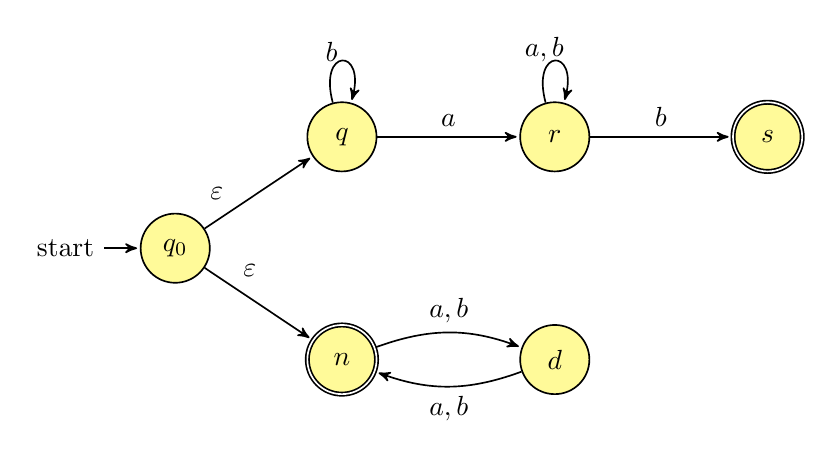
\begin{tikzpicture}[->,>=stealth',shorten >=1pt, auto, node distance=2cm, semithick]
    \tikzstyle{every state}=[text=black, fill=yellow!40]
    
    \node[initial,state] (q0)          {$q_0$};
    \node[state]         (q) [above right of=q0, xshift=20pt] {$q$};
    \node[state]         (r) [right of=q, xshift=20pt] {$r$};
    \node[state, accepting]         (s) [right of=r, xshift=20pt] {$s$};
    \node[state, accepting]         (n) [below right of=q0, xshift=20pt] {$n$};
    \node[state]         (d) [right of=n, xshift=20pt] {$d$};
    
    \path (q0) edge  [bend left=0, near start] node {$\varepsilon$} (q)
            edge [bend right=0, near start] node {$\varepsilon$} (n)
        (q) edge [bend left=0] node {$a$} (r)
            edge [loop above, near start] node {$b$} (q)
        (r) edge [bend left=0] node {$b$} (s)
            edge [loop above, near start] node {$a,b$} (r)
        (n) edge [bend left=20] node {$a,b$} (d)
        (d) edge [bend left=20] node {$a,b$} (n)
    ;
    \end{tikzpicture}
is:


\newpage

Could we do the same construction with DFA?

\vspace{50pt}

Happily, though, an analogous claim is true!

Suppose $A_1, A_2$ are languages over an alphabet $\Sigma$.
{\bf Claim:} if there is a DFA $M_1$ such that $L(M_1) = A_1$ and 
DFA $M_2$ such that $L(M_2) = A_2$, then there is another DFA, let's call it $M$, such that 
$L(M) = A_1 \cup A_2$. {\it Theorem 1.25 in Sipser, page 45}
    
    {\bf Proof idea}:
    
    
    {\bf Formal construction}: 
    
    \vfill

    
    {\bf Example}:  When $A_1 = \{w \mid w~\text{has an $a$ and ends in $b$} \}$ and 
    $A_2 = \{ w \mid w~\text{is of even length} \}$.
    
    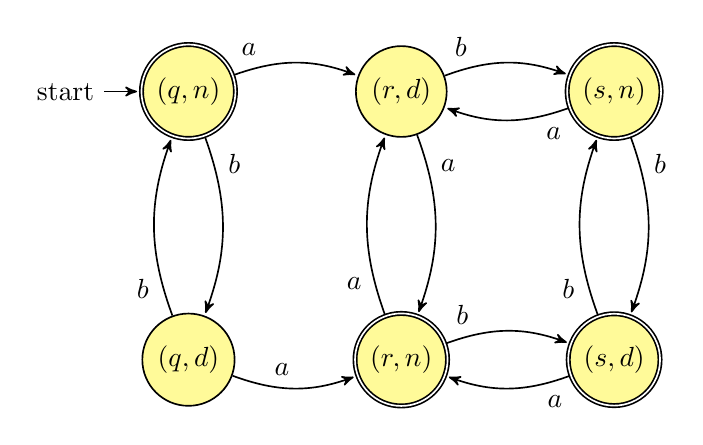
\begin{tikzpicture}[->,>=stealth',shorten >=1pt, auto, node distance=2cm, semithick]
        \tikzstyle{every state}=[text=black, fill=yellow!40]
        
        \node[initial,state,accepting] (qn)          {$(q,n)$};
        \node[state]         (qd) [below of=qn, yshift=-40pt] {$(q,d)$};
        \node[state]         (rd) [right of=qn, xshift=20pt] {$(r,d)$};
        \node[state,accepting]         (rn) [right of=qd, xshift=20pt] {$(r,n)$};
        \node[state,accepting]         (sn) [right of=rd, xshift=20pt] {$(s,n)$};
        \node[state,accepting]         (sd) [right of=rn, xshift=20pt] {$(s,d)$};
        
        \path (qn) edge  [bend left=20, near start] node {$b$} (qd)
                edge [bend left=20, near start] node {$a$} (rd)
            (qd) edge [bend left=20, near start] node {$b$} (qn)
                edge [bend right=20, near start] node {$a$} (rn)
            (rn) edge [bend left=20, near start] node {$a$} (rd)
                edge [bend left=20, near start] node {$b$} (sd)
            (rd) edge [bend left=20, near start] node {$a$} (rn)
                edge [bend left=20, near start] node {$b$} (sn)
            (sn) edge [bend left=20, near start] node {$a$} (rd)
                edge [bend left=20, near start] node {$b$} (sd)
            (sd) edge [bend left=20, near start] node {$a$} (rn)
                edge [bend left=20, near start] node {$b$} (sn)
        ;
        \end{tikzpicture}
    
    \newpage
    
    Suppose $A_1, A_2$ are languages over an alphabet $\Sigma$.
    {\bf Claim:} if there is a DFA $M_1$ such that $L(M_1) = A_1$ and 
    DFA $M_2$ such that $L(M_2) = A_2$, then there is another DFA, let's call it $M$, such that 
    $L(M) = A_1 \cap A_2$.  {\it Sipser Theorem 1.25, page 45}
    
    {\bf Proof idea}:
    
    
    {\bf Formal construction}: 
    
    \vspace{70pt}


    
    

 \vfill
\section*{Week3 wednesday}


So far we have that: 
\begin{itemize}
\item If there is a DFA recognizing a language, there is a DFA recognizing its complement.
\item If there are NFA recognizing two languages, there is a NFA recognizing their union.
\item If there are DFA recognizing two languages, there is a DFA recognizing their union.
\item If there are DFA recognizing two languages, there is a DFA recognizing their intersection.
\end{itemize}

Our goals for today are (1) prove similar results about other set operations, (2) prove that 
NFA and DFA are equally expressive, and therefore (3) define an important class of languages.

\vfill

Suppose $A_1, A_2$ are languages over an alphabet $\Sigma$.
{\bf Claim:} if there is a NFA $N_1$ such that $L(N_1) = A_1$ and 
NFA $N_2$ such that $L(N_2) = A_2$, then there is another NFA, let's call it $N$, such that 
$L(N) = A_1 \circ A_2$.

{\bf Proof idea}: Allow computation to move between $N_1$ and $N_2$ ``spontaneously" when reach an accepting state of 
$N_1$, guessing that we've reached the point where the two parts of the string in the set-wise concatenation 
are glued together.


{\bf Formal construction}: Let 
$N_1 = (Q_1, \Sigma, \delta_1, q_1, F_1)$ and $N_2 = (Q_2, \Sigma, \delta_2,q_2, F_2)$
and assume $Q_1 \cap Q_2 = \emptyset$.
Construct $N = (Q, \Sigma, \delta, q_0, F)$ where
\begin{itemize}
    \item $Q = $
    \item $q_0 = $
    \item $F = $
    \item $\delta: Q \times \Sigma_\varepsilon \to \mathcal{P}(Q)$ is defined by, for $q \in Q$ and $a \in \Sigma_{\varepsilon}$:
        \[
            \delta((q,a))=\begin{cases}  
                \delta_1 ((q,a)) &\qquad\text{if } q\in Q_1 \textrm{ and } q \notin F_1\\ 
                \delta_1 ((q,a)) &\qquad\text{if } q\in F_1 \textrm{ and } a \in \Sigma\\ 
                \delta_1 ((q,a)) \cup \{q_2\} &\qquad\text{if } q\in F_1 \textrm{ and } a = \varepsilon\\ 
                \delta_2 ((q,a)) &\qquad\text{if } q\in Q_2
            \end{cases}
        \]
\end{itemize}

\vfill

{\it Proof of correctness would prove that $L(N) = A_1 \circ A_2$ by considering
an arbitrary string accepted by $N$, tracing an accepting computation of $N$ on it, and using 
that trace to prove the string can be written as the result of concatenating two strings, 
the first in $A_1$ and the second in $A_2$; then, taking an arbitrary 
string in $A_1 \circ A_2$ and proving that it is accepted by $N$. Details left for extra practice.}

\newpage



Suppose $A$ is a language over an alphabet $\Sigma$.
{\bf Claim:} if there is a NFA $N$ such that $L(N) = A$, then there is another NFA, let's call it $N'$, such that 
$L(N') = A^*$.

{\bf Proof idea}: Add a fresh start state, which is an accept state. Add spontaneous 
moves from each (old) accept state to the old start state.

{\bf Formal construction}: Let 
$N = (Q, \Sigma, \delta, q_1, F)$ and assume $q_0 \notin Q$.
Construct $N' = (Q', \Sigma, \delta', q_0, F')$ where
\begin{itemize}
    \item $Q' = Q \cup \{q_0\}$
    \item $F' = F \cup \{q_0\}$
    \item $\delta': Q' \times \Sigma_\varepsilon \to \mathcal{P}(Q')$ is defined by, for $q \in Q'$ and $a \in \Sigma_{\varepsilon}$:
        \[
            \delta'((q,a))=\begin{cases}  
                \delta ((q,a)) &\qquad\text{if } q\in Q \textrm{ and } q \notin F\\ 
                \delta ((q,a)) &\qquad\text{if } q\in F \textrm{ and } a \in \Sigma\\ 
                \delta ((q,a)) \cup \{q_1\} &\qquad\text{if } q\in F \textrm{ and } a = \varepsilon\\ 
                \{q_1\} &\qquad\text{if } q = q_0 \textrm{ and } a = \varepsilon \\
                \emptyset &\qquad\text{if } q = q_0 \textrm { and } a \in \Sigma
            \end{cases}
        \]
\end{itemize}


{\it Proof of correctness would prove that $L(N') = A^*$ by considering
an arbitrary string accepted by $N'$, tracing an accepting computation of $N'$ on it, and using 
that trace to prove the string can be written as the result of concatenating some number of strings, 
each of which is in $A$; then, taking an arbitrary 
string in $A^*$ and proving that it is accepted by $N'$. Details left for extra practice.}


{\bf Application}: A state diagram for a NFA over $\Sigma = \{a,b\}$ 
that recognizes $L (( a^*b)^* )$:

\vfill
\newpage
Suppose $A$ is a language over an alphabet $\Sigma$.
{\bf Claim:} if there is a NFA $N$ such that $L(N) = A$ then 
there is a DFA $M$ such that $L(M) = A$.

{\bf Proof idea}: States in $M$ are ``macro-states" -- collections of states from $N$ -- 
that represent the set of possible states a computation of $N$ might be in.


{\bf Formal construction}: Let $N = (Q, \Sigma, \delta, q_0, F)$.  Define 
\[
M = (~ \mathcal{P}(Q), \Sigma, \delta', q',  \{ X \subseteq Q \mid X \cap F \neq \emptyset \}~ )
\]
where $q' = \{ q \in Q \mid \text{$q = q_0$ or is accessible from $q_0$ by spontaneous moves in $N$} \}$
and 
\[
    \delta' (~(X, x)~) = \{ q \in Q \mid q \in \delta( ~(r,x)~) ~\text{for some $r \in X$ or is accessible 
from such an $r$ by spontaneous moves in $N$} \}
\]


Consider the state diagram of an NFA over $\{a,b\}$. Use the ``macro-state'' construction 
to find an equivalent DFA.

\includegraphics[width=2.5in]{Lect6NFA1.png}




\vfill

Consider the state diagram of an NFA over $\{0,1\}$. Use the ``macro-state'' construction 
to find an equivalent DFA.


\includegraphics[width=1.8in]{Lect6NFA2.png}


\vfill

Note: We can often prune the DFAs that result from the ``macro-state'' constructions to get an 
equivalent DFA with fewer states (e.g.\ only the ``macro-states" reachable from the start state).

\newpage


{\bf The class of regular languages}

Fix an alphabet $\Sigma$. For each language $L$ over $\Sigma$:
\begin{center}
\begin{tabular}{cc}
    {\bf There is a DFA over $\Sigma$ that recognizes $L$}&$\exists M ~(M \textrm{ is a DFA and } L(M) = A)$\\
    {\it if and only if}&\\
    {\bf There is a NFA over $\Sigma$ that recognizes $L$}&$\exists N ~(N \textrm{ is a NFA and } L(N) = A)$\\
    {\it if and only if}&\\
    {\bf There is a regular expression over $\Sigma$ that describes $L$} &$\exists R ~(R \textrm{ is a regular expression and } L(R) = A)$\\
\end{tabular}
\end{center}

A language is called {\bf regular} when any (hence all) of the above three conditions are met.

We already proved that DFAs and NFAs are equally expressive. It remains to prove that regular expressions 
are too.

Part 1: Suppose $A$ is a language over an alphabet $\Sigma$.
If there is a regular expression $R$ such that $L(R) = A$, then there is a NFA, let's call it $N$, such that 
$L(N) = A$.

{\bf Structural induction}: Regular expression is built from basis regular expressions using inductive steps
(union, concatenation, Kleene star symbols). Use constructions to mirror these in NFAs.


{\bf Application}: A state diagram for a NFA over $\{a,b\}$ that recognizes $L(a^* (ab)^*)$:

\vfill

Part 2: Suppose $A$ is a language over an alphabet $\Sigma$.
If there is a DFA $M$ such that $L(M) = A$, then there is a regular expression, let's call it $R$, such that 
$L(R) = A$.

{\bf Proof idea}: Trace all possible paths from start state to accept state.  Express labels of these paths
as regular expressions, and union them all.

\begin{enumerate}
\item Add new start state with $\varepsilon$ arrow to old start state.
\item Add new accept state with $\varepsilon$ arrow from old accept states.  Make old accept states
non-accept.
\item Remove one (of the old) states at a time: modify regular expressions on arrows that went through removed
state to restore language recognized by machine.
\end{enumerate}

{\bf Application}: Find a regular expression describing the language recognized by the DFA with 
state diagram

\includegraphics[width=2.5in]{Lect6NFA3.png}

\vfill
 \vfill
\section*{Week2 wednesday}



{\bf Review}: Formal definition of finite automaton: $M = (Q, \Sigma, \delta, q_0, F)$ 

\begin{center}
\begin{multicols}{2}
\begin{itemize}
\setlength{\itemsep}{2pt}
\item Finite set of states $Q$
\item Alphabet $\Sigma$
\item Transition function $\delta$
\item Start state $q_0$
\item Accept (final) states $F$
\end{itemize}
\end{multicols}
\end{center}
In the state diagram of $M$, how many outgoing arrows are there from each state?

$M = ( \{ q, r, s\}, \{a,b\}, \delta, q, \{q\} )$ 
where $\delta$ is  (rows labelled by states
and columns labelled by symbols):
\begin{center}
\begin{tabular}{c|cc}
$\delta$ & $a$ & $b$ \\
\hline
$q$ & $r$ & $r$ \\
$r$ & $s$ & $s$ \\
$s$ & $q$ & $q$ \\
\end{tabular}
\end{center}

The state diagram for $M$ is 

\vfill



Give two examples of strings that are accepted by $M$ and two examples of strings that are rejected by $M$:

\vfill



$L(M) = $

A regular expression describing $L(M)$ is




\newpage
Let the alphabet be $\Sigma_1 = \{0,1\}$.

A state diagram for a finite automaton that recognizes $\{w \in \Sigma_1^* \mid w~\text{contains at most two $1$'s} \}$ is

\vfill

A state diagram for a finite automaton that recognizes $\{w \in \Sigma_1^* \mid w~\text{contains more than two $1$'s} \}$ is

\vfill

\textbf{Strategy}: Add ``labels" for states in the state diagram, e.g. 
``have not seen any of desired pattern yet'' or ``sink state''.
Then, we can use the analysis of the roles of the states in the state diagram to work towards a 
description of the language recognized by the finite automaton. 

\vfill
A useful bit of terminology: the {\bf iterated transition function} of a finite automaton
$M = (Q, \Sigma, \delta, q_0, F)$ is defined recursively by
\[
\delta^* (~(q,w)~) 
=\begin{cases}
q  \qquad &\text{if $q \in Q, w = \varepsilon$} \\
\delta( ~(q,a)~) \qquad &\text{if $q \in Q$, $w = a \in \Sigma$ } \\
\delta(~(\delta^*(q,u), a) ~) \qquad &\text{if $q \in Q$, $w = ua$ where $u \in  \Sigma^*$ and $a \in \Sigma$}
\end{cases}
\]

Using  this terminology, $M$ accepts a string $w$ over $\Sigma$ if and only if $\delta^*( ~(q_0,w)~) \in F$.

\newpage
Suppose $A$ is a language over an alphabet $\Sigma$. By definition, this means $A$ is a subset of $\Sigma^*$.
{\bf Claim:} if there is a DFA $M$ such that $L(M) = A$ then there is another DFA, let's call it $M'$, such that 
$L(M') = \overline{A}$, the complement of $A$, defined as $\{ w \in \Sigma^* \mid w \notin A \}$.

{\bf Proof idea}:


{\bf Proof}: 




\vfill

Application: Design a finite automaton that recognizes the language of all strings over $\{a,b\}$
whose length is not a multiple of $3$.

\vfill

{\bf Note}: On Friday, we'll see a new kind of finite automaton. It will be helpful to distinguish it from the
machines we've been talking about so we'll use {\bf Deterministic Finite Automaton} (DFA) to refer to the machines 
from Section 1.1. \vfill
\section*{Week2 friday}



\begin{center}
\begin{tabular}{|ll|}
\hline
\multicolumn{2}{|l|}{{\bf Nondeterministic finite automaton}  (Sipser Page 53) Given as $M = (Q, \Sigma, \delta, q_0, F)$}\\
& \\
Finite set of states $Q$  & Can  be labelled by any collection  of distinct names. Default: $q0, q1, \ldots$  \\
Alphabet $\Sigma$ &  Each input to the automaton is a string over  $\Sigma$. \\
Arrow labels $\Sigma_\varepsilon$ &  $\Sigma_\varepsilon = \Sigma \cup \{ \varepsilon\}$. \\
&  Arrows 
in the state diagram are labelled either by symbols from $\Sigma$ or by $\varepsilon$ \\
Transition function $\delta$  & $\delta: Q \times \Sigma_{\varepsilon} \to \mathcal{P}(Q)$
gives the {\bf set of possible next states} for a transition \\
&  from the current state upon reading a symbol or spontaneously moving.\\
Start state $q_0$ & Element of $Q$.  Each computation of the machine starts at the  start  state.\\
Accept (final) states $F$ & $F \subseteq  Q$.\\
& \\
\multicolumn{2}{|p{\textwidth}|}{$M$ accepts the input string $w \in \Sigma^*$ if and only if {\bf there is} a computation of $M$ on 
$w$ that processes the whole string and ends in an
accept state.}\\
\hline
\end{tabular}
\end{center}

The formal definition of the NFA over $\{0,1\}$ given by this state diagram is: 

\includegraphics[width=2in]{Lect4NFA1.png}

The language over $\{0,1\}$ recognized by this NFA is:

\vspace{70pt}

Change the transition function to get a different NFA which accepts
the empty string (and potentially other strings too).


\newpage

The state diagram of an NFA over $\{a,b\}$ is below.  The formal definition of this NFA is:

\vspace{-30pt}

\includegraphics[width=2.5in]{Lect5NFA1.png}


\vspace{-10pt}

The language recognized by this NFA is:  \vfill
\section*{Week1 friday}


{\bf Review}: Determine whether each statement below about regular expressions
over the alphabet $\{a,b,c\}$ is true or false:

\begin{comment}
True or False: \qquad 
   $a  \in L(~(a \cup b )~\cup c)$
\end{comment}

True or False: \qquad 
   $ab  \in L(~ (a \cup b)^*  ~)$
   
True or False: \qquad    
   $ba \in L( ~ a^* b^* ~)$
   
True or False: \qquad 
   $\varepsilon  \in L(a \cup b \cup c)$
   
True or False: \qquad 
   $\varepsilon  \in L(~ (a \cup b)^*  ~)$

True or False: \qquad 
   $\varepsilon \in L( ~ aa^* \cup bb^* ~)$


**This definition was in the pre-class reading**
A finite automaton (FA) is specified by  $M = (Q, \Sigma, \delta, q_0, F)$.
This $5$-tuple is called the {\bf formal definition} of the FA. The FA can also 
be represented by its state diagram: with nodes for the state, labelled edges specifying the 
transition function, and decorations on nodes denoting the start and accept states.

\begin{quote}
Finite set of states $Q$ can be labelled by any collection of distinct names. Often
we use default state labels $q0, q1, \ldots$ 
\end{quote}

\begin{quote}  
The alphabet $\Sigma$ determines the possible inputs to the automaton. 
Each input to the automaton is a string over  $\Sigma$, and the automaton ``processes'' the input
one symbol (or character) at a time.
\end{quote}

\begin{quote}
The transition function $\delta$ gives the next state of the automaton based on the current state of 
the machine and on the next input symbol.
\end{quote}

\begin{quote}
The start state $q_0$ is an element of $Q$.  Each computation of the machine starts at the  start  state.
\end{quote}

\begin{quote}
The accept (final) states $F$ form a subset of the states of the automaton, $F \subseteq  Q$. 
These states are used to flag if the machine accepts or rejects an input string.
\end{quote}


\begin{quote}
The computation of a machine on an input string is a sequence of states
in the machine,  starting with the start state, determined by transitions 
of the machine as it reads successive input symbols.
\end{quote}

\begin{quote}
The finite automaton $M$ accepts the given input string exactly when the computation of $M$ on the input string
ends in an accept state. $M$ rejects the given input string exactly when the computation of 
$M$ on the input string ends in a nonaccept state, that is, a state that is not in $F$.
\end{quote}

\begin{quote} 
The language of $M$, $L(M)$, is defined as the set of  all strings that are each accepted 
by the machine $M$. Each string that is rejected by $M$ is not in $L(M)$.
The language of $M$ is also called the language recognized by $M$.
\end{quote}   
   
What is {\bf finite} about all finite automata? (Select all that apply)
\begin{itemize}
   \item[$\square$] The size of the machine (number of states, number of arrows)
   \item[$\square$] The length of each computation of the machine
   \item[$\square$] The number of strings that are accepted by the machine
\end{itemize}
  
\begin{figure}[h]
   \centering
   \includegraphics[width=3in]{Lect2DFA1.png} 
\end{figure}
   
The formal definition of this FA is
   
\vspace{100pt}
   

Classify each string $a, aa, ab, ba, bb, \varepsilon$ as accepted by the FA or rejected by the FA.  

{\it Why are these the only two options?}

\vspace{200pt}


The language recognized by this automaton is
  
\vspace{100pt}
   

\begin{figure}[h]
  \centering
  \includegraphics[width=3in]{Lect2DFA2.png} 
\end{figure}
   

The language recognized by this automaton is
  
\vspace{100pt}

\begin{figure}[h]
    \centering
    \includegraphics[width=3in]{Lect2DFA3.png} 
\end{figure}

The language recognized by this automaton is
  
\vspace{100pt}
 \vfill
\end{document}